\documentclass{article}

\usepackage{amsmath}
\usepackage{fancyhdr}
\usepackage{graphicx}
\graphicspath{{}}

%% some colours
\usepackage{color}
\definecolor{deepblue}{rgb}{0,0,0.5}
\definecolor{deepred}{rgb}{0.6,0,0}
\definecolor{deepgreen}{rgb}{0,0.5,0}
\definecolor{backcolour}{rgb}{0.95,0.96,0.93}

%%%%%%%%%%%%%% CODE STUFF %%%%%%%%%%%%%%
%%%%%%%%%%%%%%%%%%%%%%%%%%%%%%%%%%%%%%%%
\usepackage{cprotect} % to be used in sol
\usepackage{listings} % for code display
% setting code style
\newcommand\pythonstyle{\lstset{
        language=Python,
        backgroundcolor=\color{backcolour},
		basicstyle=\footnotesize,
		otherkeywords={self},
		keywordstyle=\footnotesize\color{deepblue},
		emph={__init__},
		emphstyle=\footnotesize\color{deepred},
		stringstyle=\color{deepgreen},
		frame=single,
		showstringspaces=false  ,
		breaklines=true,
		numbers=left,
		numberstyle=\footnotesize,
		tabsize=4,
		breakatwhitespace=false
	}}

% Python environment
\lstnewenvironment{python}[1][]{
    \pythonstyle
    \lstset{#1}
}{}

% Python for external files
\newcommand\pythonexternal[2][]{{
    \pythonstyle
    \lstinputlisting[#1]{#2}
}}

% Python for inline
\newcommand\pythoninline[1]{{\pythonstyle\lstinline!#1!}}

%%%%%%%%%%%%%%%%%%%%%%%%%%%%%%%%%%%%%%%%
% setting the style for ex documents
\pagestyle{fancy}
\fancyhf{}
\fancyhead[L]{\thetitle}
\fancyhead[C]{}
\fancyhead[R]{\theauthor}
\renewcommand{\headrulewidth}{0.4pt} %obere Trennlinie
\fancyfoot[L]{Due: \thedate}
\fancyfoot[R]{\thepage} %Seitennummer
\renewcommand{\footrulewidth}{0.4pt}

% include solutions
\newcommand\sol[1]{{\large\textbf{\\Solution:}}#1}


\title{BPP Exercise 3 - Directing the Flow}
\author{A. Hain, M. Nipshagen}
\date{23.04.2018, 8:00}

\makeatletter
\let\thetitle\@title
\let\theauthor\@author
\let\thedate\@date
\makeatother

% do not include solutions
\renewcommand\sol[1]{}

\begin{document}

The deadline for this exercise sheet is \textbf{Monday, \thedate.}
%
%\section*{Introductory Words}
%In case we have some information that doesn't directly concern the current exercises.
%
\section{Boolean Operators}
Determine the truth values of the following boolean operators for each configuration
of truth values as given in the tables

\subsection{}
\begin{tabular}{| c | c | c | c |}
  \hline
  \textbf{a} & \textbf{b} & \textbf{c} & \textbf{(b or c) and (a or c)} \\
  \hline
  true & true & true & \sol{true} \\
  \hline
  true & true & false & \sol{true} \\
  \hline
  true & false & true & \sol{true} \\
  \hline
  true & false & false & \sol{false} \\
  \hline
  false & true & true & \sol{true} \\
  \hline
  false & true & false & \sol{false} \\
  \hline
  false & false & true & \sol{true} \\
  \hline
  false & false & false & \sol{false} \\
  \hline
\end{tabular}

\subsection{}
\begin{tabular}{| c | c | c | c |}
  \hline
  \textbf{a} & \textbf{b} & \textbf{c} & \textbf{a or (b and c) and (not c or not a)} \\
  \hline
  true & true & true & \sol{true} \\
  \hline
  true & true & false & \sol{true} \\
  \hline
  true & false & true & \sol{true} \\
  \hline
  true & false & false & \sol{true} \\
  \hline
  false & true & true & \sol{true} \\
  \hline
  false & true & false & \sol{false} \\
  \hline
  false & false & true & \sol{false} \\
  \hline
  false & false & false & \sol{false} \\
  \hline  
\end{tabular}

\subsection{}
\begin{tabular}{| c | c | c | c |}
  \hline
  \textbf{a} & \textbf{b} & \textbf{c} & \textbf{not(not(b and not(c or a)))} \\
  \hline
  true & true & true & \sol{false} \\
  \hline
  true & true & false & \sol{false} \\
  \hline
  true & false & true & \sol{false} \\
  \hline
  true & false & false & \sol{false} \\
  \hline
  false & true & true & \sol{false} \\
  \hline
  false & true & false & \sol{true} \\
  \hline
  false & false & true & \sol{false} \\
  \hline
  false & false & false & \sol{false} \\
  \hline
\end{tabular}

\section{Warm up -- Prof Strikes Again}
Remember the task from last week? Now that your prof computed your numerical grade, the
functionality of this program shall be extended by automatically determining whether
someone passed the class or not based on this grade.\\
Write a function \texttt{passed} that takes a grade
as a parameter and returns whether the student passed or failed.

\cprotect\sol{
\begin{python}
def passed(grade):
  return grade <= 4.0
\end{python}
}

\section{Loops}

\subsection{N Bottles of Beer}
Similar to Hello World programs, 99 bottles programs give us an idea of how
a programming language looks as they show the basic loop concepts.
The 99 bottles program “sings” a little song which goes like this:\\\\
\textit{
99 bottles of beer on the wall, 99 bottles of beer. Take one down and
pass it around, 98 bottles of beer on the wall.\\
98 bottles of beer on the wall, 98 bottles of beer. Take one down and
pass it around, 97 bottles of beer on the wall.\\
. . .\\
1 bottle of beer on the wall, 1 bottle of beer. Take one down and
pass it around, no more bottles of beer on the wall.\\\\
}
Write a function \texttt{n\_bottles(n)} in the script \texttt{n\_bottles.py} which
sings the song starting with n bottles instead of 99. If n is bigger than 99 or
smaller than 5 print a message that you want to sing a funnier song than n bottles
(of course replace n with the current n). Your final result may also structure
the verses in a different layout.

\cprotect\sol{
\begin{python}
def bottles(n):
    """Formats plural according to number of bottles."""
    return ('1 bottle' if n == 1 else str(n) + ' bottles') + ' of beer'

def n_bottles(n):
    """
    Go through the bottles of beer on the wall, and pass them around.

    Calls `bottles(n)` for formatting, and reduces n by 1 each iteration
    """
    if 5 <= n <= 99:
        while(n > 0):
            print(bottles(n) + ' on the wall,\n  ' + bottles(n) + '.')
            n = n - 1
            print('Take one down and pass it around,\n  ' +
                # conditional expression to determine whethere there are bottles left
                bottles(n if n > 0 else 'no more') + 
                ' on the wall.\n')
    else:
        print('I want to sing funnier songs than "' + bottles(n) + '".\n')


n_bottles(3)
n_bottles(1011)
n_bottles(5)
\end{python}
Output:
\texttt{
\small{\\
I want to sing funnier songs than "3 bottles of beer".\\\\
I want to sing funnier songs than "1011 bottles of beer".\\\\
5 bottles of beer on the wall,\\
\indent 5 bottles of beer.\\
Take one down and pass it around,\\
\indent 4 bottles of beer on the wall.\\\\
4 bottles of beer on the wall,\\
\indent 4 bottles of beer.\\
Take one down and pass it around,\\
\indent 3 bottles of beer on the wall.\\\\
3 bottles of beer on the wall,\\
\indent 3 bottles of beer.\\
Take one down and pass it around,\\
\indent 2 bottles of beer on the wall.\\\\
2 bottles of beer on the wall,\\
\indent 2 bottles of beer.\\
Take one down and pass it around,\\
\indent 1 bottle of beer on the wall.\\\\
1 bottle of beer on the wall,\\
\indent 1 bottle of beer.\\
Take one down and pass it around,\\
\indent no more bottles of beer on the wall.\\
}
}
}


\subsection{Return of the turtle}
\FloatBarrier
You hopefully remember the turtle from the first week -- you drew a Saint Nicholas' house with it.
This time we will draw even more houses! And some trees to keep them company.\\
Write a script \texttt{turtle\_world.py}. Develop a function \texttt{draw\_house} that draws a house --
it doesn't need to be the Saint Nicholas' house, but you can recylce your code if you like.
Then write a function \texttt{draw\_tree{height}} that draws a tree of a given "height".
The height serves a double purpose as the branching factor of the tree. Your tree is going to be a fractal,
which means that it will be a pattern that repeats itself recursively.

\begin{figure}[h]
  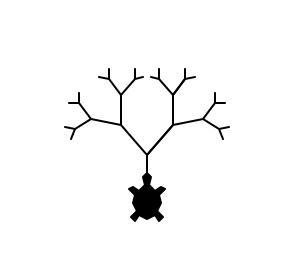
\includegraphics[scale=0.8]{recursive_tree}
  \caption{Example Tree}
  \label{fig:tree:1}
\end{figure}


\noindent To build the tree follow this algorithm:\\
\begin{lstlisting}
To draw a tree with height h:
  If height h is 0, stop.
  Draw a line of length L * h.
  Rotate left by angle A.
  Draw a tree of height h - 1.
  Rotate right by angle 2A.
  Draw a tree of height h - 1.
  Rotate left by angle A.
  Move back to the beginning of the line.
\end{lstlisting}

\noindent The resulting tree should look similar to Figure \ref{fig:tree:1}. Choose $A$ and $L$ as you like, be creative!\\
Now draw a simple landscape. Draw a house, a small tree, a big tree, a small tree, and repeat this pattern a couple of times
(Figure \ref{fig:world:flat}). Or build a different one. Just make it repetitive (Yes, use loops).

\begin{figure}[h]
	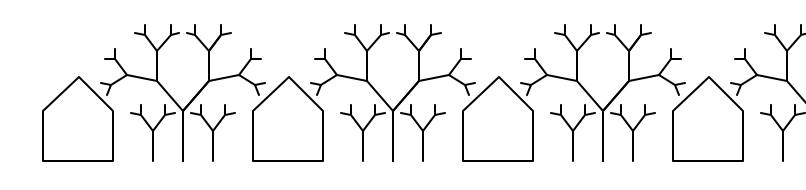
\includegraphics[width=\textwidth]{flat_world}
	\caption{Flat World}
	\label{fig:world:flat}
\end{figure}

\noindent\textbf{Bonus}: Can you build a round world like in Figure \ref{fig:world:round}?

\begin{figure}[h]
	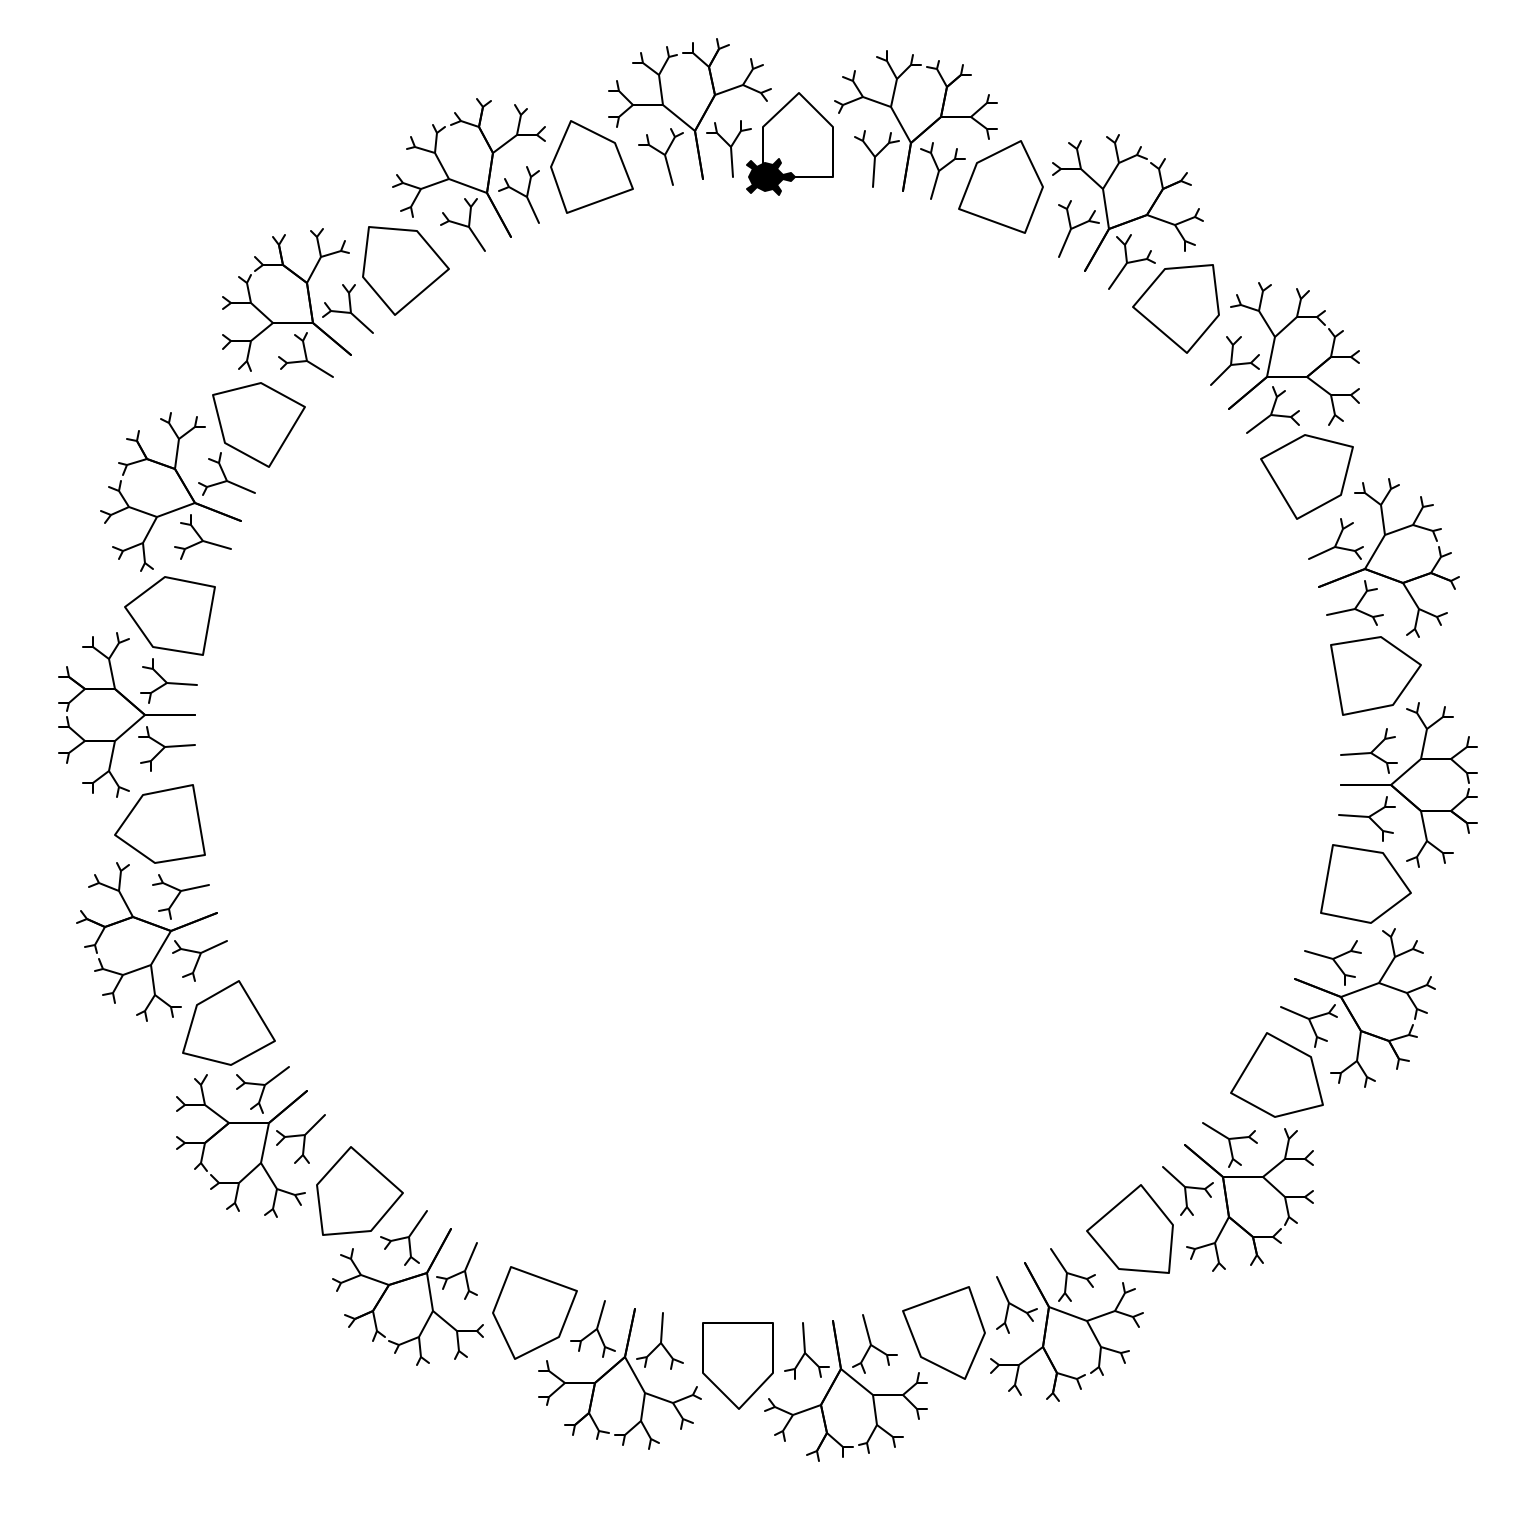
\includegraphics[width=\textwidth]{round_world}
	\caption{Round World}
	\label{fig:world:round}
\end{figure}

\cprotect\sol{
\begin{python}

\end{python}
}

\end{document}
